\documentclass[11pt, a4paper]{article}

% Encoding
\usepackage[utf8]{inputenc}

% Hyphenation
\usepackage[english]{babel}

% Extended math environments
\usepackage{amsmath}
\numberwithin{equation}{section}

% Additional math fonts and symbols
\usepackage{amsfonts}
\usepackage{amssymb}

% Units and uncertainties
\usepackage{siunitx}
\sisetup{
    separate-uncertainty
}

% Margins
\usepackage[left=3.5cm, right=3.5cm, top=3cm, bottom=3cm, twoside]{geometry}

% Pictures
\usepackage{graphicx}

% Hyperlinks
\usepackage{hyperref}
\hypersetup{
    colorlinks = true,
    allcolors = {black}
}

% Better table layouts
\usepackage{booktabs}
\usepackage{multirow}
\usepackage{multicol}

% Page Header
\usepackage{fancyhdr}

% Float Barriers
\usepackage{placeins}

% Rotated figures
\usepackage{caption}
\usepackage{subcaption}
\usepackage{rotating}

% Wrapped figures
\usepackage{wrapfig}

\usepackage{float}

% Caption-Setup
\captionsetup{font={small}}
\renewcommand{\thefigure}{\thesection.\arabic{figure}}
\renewcommand{\thesubfigure}{\alph{subfigure}}
\renewcommand{\thetable}{\thesection.\arabic{table}}
\renewcommand{\thesubtable}{\alph{subtable}}

% Depth of TOC (Level: 1 sections, 2 subsections, 3 subsubsections)
\setcounter{tocdepth}{3}

% FANCYHDR SETUP
\pagestyle{fancy}
\fancyhead[EL,OR]{\thepage}
\fancyhead[ER]{\leftmark}
\fancyhead[OL]{\rightmark}

\renewcommand{\sectionmark}[1]{
\markboth{\thesection{} #1}{\thesection{} #1}
}
\renewcommand{\subsectionmark}[1]{
\markright{\thesubsection{} #1}
}

% Document Info
\title{Particles in a potential}

\author{Christopher Deutsch\footnote{christopher.deutsch@uni-bonn.de} \and Philip Hauer\footnote{philiphauer@googlemail.com}}

\date{\today}

\begin{document}

\begin{titlepage}

\maketitle

% ABSTRACT
\begin{abstract}
\noindent 
We consider a set of two oppositely charged particles that interact via a two-particle potential in a finite volume in two dimensions. With a Random-Walk Metropolis algorithm we simulate the time evolution of this system. Our focus lies on the analysis of the temperature dependence in particular the average pair distance. Additionally we also study the behavior for different potentials and in three dimensions.
\end{abstract}

\end{titlepage}

% TABLE OF CONTENTS
\tableofcontents
% New page after TOC
\newpage

% CONTENT

\section{Introduction}
This paper summarizes our results of the analysis of a two-dimensional system where we only have two kind of particles, a positive and a negative one. They interact via a potential which is given by
\begin{equation}
V_{ij} = \frac{q_i q_j}{\left| \vec{r}_i - \vec{r}_j \right|} + \frac{1}{\left| \vec{r}_i - \vec{r}_j \right|^8} \, .
\end{equation}
For the analysis we use a Random-Walk Metropolis algorithm which will be explained in chapter \ref{Sec:Metropolis}. The used algorithm depends on the temperature and we study this dependence in chapter \ref{Sec:Temperature}. As an indicator for the phase of the system we monitor the average pair distance. A visualization of the different phases was also done and can be found in the section \ref{Sec:Visualisation}. In addition to that we did some further research with other potentials (e.g. Lennard-Jones potential) and we simulated the system in three dimensions. These further thoughts and results are explained in chapter \ref{Sec:Further_Analysis}.

\section{Canonical ensemble} \label{Sec:Canonical_Ensemble}

The statistical ensemble describing a fixed number of particles~$N$ in a given volume~$V$, which is in thermal equilibrium with a heat bath of temperature~$T$, is the canonical ensemble.
Aim of this project is to sample states from a given ensemble with fixed $N, V, T$ and use these to calculate expectation values of certain observables.
For this the probability density for realizing a specific microstate of the ensemble needs to be known.
In statistical mechanics the probability density for a canonical ensemble to be in a microstate with energy eigenvalue~$E$ is given by \cite{schwabl}
\begin{align*}
	P = \frac{1}{Z} \exp\left[ -\beta E \right]
\end{align*}
with the normalization factor $1/Z$, where $Z$ is the canonical partition function.
For a system of particles with an inter-particle potential~$V_{ij}$ and neglecting kinetic energies the canonical partition function
\begin{align*}
	Z = \int \prod_{i=1}^N \mathrm{d}\mathbf{r}_i \exp\left[ -\beta \sum_{i < j} V_{ij} \right]
\end{align*}
is a constant of the ensemble and the total energy of the system is
\begin{align*}
	E = \sum_{i < j} V_{ij} \text{.}
\end{align*}
Since the calculation of $Z$ is computationally expensive a sampling method without the need of a normalized probability density is desirable.
One such method is sampling using the Metropolis algorithm, which is introduced in the following section.

\section{Metropolis algorithm} \label{Sec:Metropolis}


\section{Temperature dependence} \label{Sec:Temperature}

\begin{figure}
	\centering
	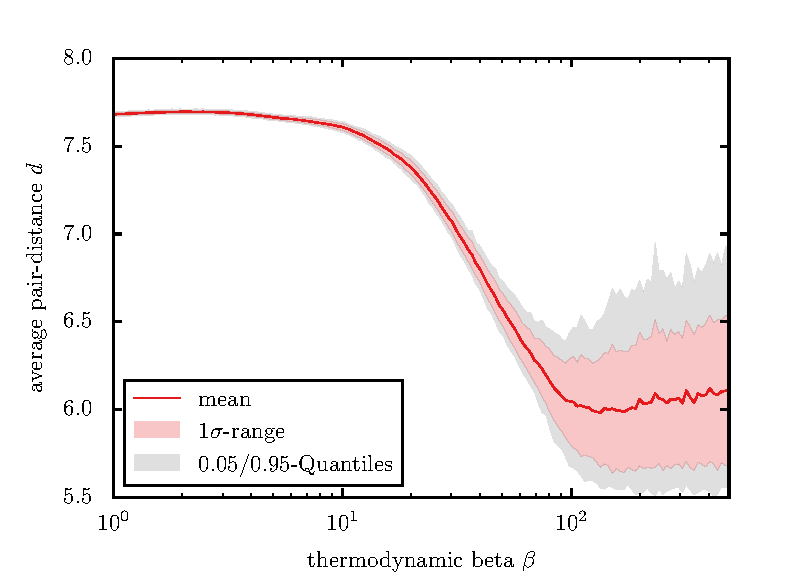
\includegraphics{./figures/temp_dep_coulomb2d.pdf}
	\caption{Temperature dependence}
\end{figure}


\section{Visualization} \label{Sec:Visualisation}
\section{Further Analysis} \label{Sec:Further_Analysis}

\FloatBarrier
% BIBLIOGRAPHY
\vspace{\fill}
\begin{thebibliography}{9}
\bibitem{schwabl}
	F. Schwabl,
	\emph{Statistische Mechanik},
	Springer, Berlin, 3rd edition 2006.
\end{thebibliography}
\end{document}